\documentclass{article}

% Language setting
% Replace `english' with e.g. `spanish' to change the document language
\usepackage[english,russian]{babel}
\usepackage{amsmath}

%графика
\usepackage{wrapfig}
\usepackage{graphicx}
\usepackage{pgfplots}
\usepackage{tikz}


\usepackage{tcolorbox}

% Set page size and margins
% Replace `letterpaper' with `a4paper' for UK/EU standard size
\usepackage[letterpaper,top=2cm,bottom=2cm,left=3cm,right=3cm,marginparwidth=1.75cm]{geometry}

% Useful packages
\usepackage{amsmath}
\usepackage{amssymb}
\usepackage{graphicx}
\usepackage{fixltx2e}
\usepackage[colorlinks=true, allcolors=blue]{hyperref}

\usepackage{geometry}
\geometry{left=25mm,right=25mm,
 top=25mm,bottom=25mm}


\begin{document}
\begin{titlepage}
    \begin{center}
        \line(1,0){300}\\
        [0,25in]
        \huge{\bfseries Linear Regression. Линейная регрессия.}\\
        [2mm]
         \line(1,0){300}\\
         \textsc{\Large Data Science.}\\
         \textsc{\Large Lectures. Week 1.}\\
         [4mm]
          \textsc{\small Polina Kravets \\
          20 сентября 2022 г.\\}
    \end{center}

\tableofcontents
\end{titlepage}



\section{Регрессионный анализ в эконометрике}\label{sec:intro}
\textbf{Регрессионный анализ} - исследование зависимости одной переменной от другой.
\begin{itemize}
    \item Зависимая переменная - переменная, изменение которой хотим объяснить. 
    \item Переменные, с помощью которых объясняем эти изменения, называются независимыми, или факторами.
\end{itemize}
\textbf{Облако рассеивания} - инструмент, с помощью которого можно оценить вид зависимости.\\

\begin{wrapfigure}{r} {0.55\textwidth}
    \centering
    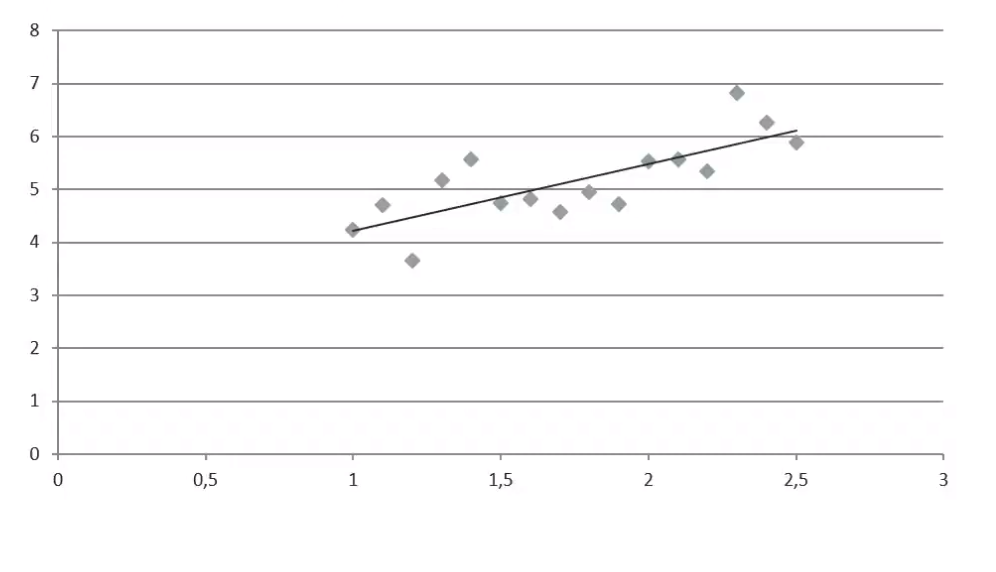
\includegraphics[width=0.55\textwidth]{graph1.png}
    \caption[Optional caption]{Пример облака рассеивания}
    \label{fig:example_chart}
\end{wrapfigure}

\textbf{Простая точечная диаграмма для двух переменных}: 
\begin{itemize}
    \item у - зависимая переменная, вертикальная ось;
    \item х - независимая переменная, горизонтальная ось. 
\end{itemize}
 
Каждая точка представляет собой пару наблюдений (х;у).

Проведенная прямая - попытка оценить, является ли зависимость (х;у) линейной; насколько далеко ложатся точки от данной прямой.

\textit{Визуально по облаку рассеивания можно оценить зависимость и вид зависимости.}

Если имеет место линейная зависимость (х;у), то облако будет сильно вытянутым. Если облако имеет круглую форму - линейная зависимость отсутствует. 
\begin{itemize}
    \item В зависимости от того, как располагается прямая, близко к которой располагаются точки, можно понять, какому изменению переменной у будет соответствовать изменение переменной х;
    \item Прямая направлена вверх → рост одной переменной соответствует росту другой переменной; вниз → противоположно;
    \item \textbf{\textit {Важно помнить, что этот визуальный инструмент не дает никаких математических вычислений и позволяет лишь выдвигать гипотезы о зависимости у от х.}}
\end{itemize}

\section{Уравнение регрессии}\label{sec:reg-eq}
Математически уравнение регрессии, выражающее зависимость у от х, представляет собой:
\[Y_i = f(T, X_i, \varepsilon_i)\]
где Y\textsubscript{i} - объясняемая переменная, X\textsubscript{i} - объясняющая переменная (фактор), \textit{f} - определяет модель регрессии, \textit{T} - набор параметров модели, \(\varepsilon_i\textnormal{- случайные ошибки.}\)

\textbf{\textit {Если функция f линейна, то соответствующая регрессия называется линейной.}}

Это можно записать в виде условного математического ожидания:
\[E(Y_i\textbar X_i) = B_0 + B_1X_i\]
где \(B_0\) - у-пересечение (intercept-term), \(B_1\) - коэффициент наклона.

Без использования условного математического ожидания:
\[Y_i = B_0 + B_1X_i + \varepsilon_i\]

Нужно выбрать модель регрессии так, чтобы она адекватно описывала зависимость у от х.

\(\varepsilon_i\) - независимая случайная величина с нулевым математическим ожиданием, имеет нормальное распределение.

\subsection{Выборочное уравнение в линейной регрессии}
На практике имеется реализация выборки, т.е. точные значения коэффициентов \(B_0\) и \(B_1\) неизвестны.

Выборочное уравнение линейной регрессии:
\[Y_i = b_1X_i + b_0 + e_i\]
\(b_0\), \(b_1\) отличаются от истинных значений, \(e_i = Y_i - b_0 - b_1X_i \) - остатки,  \(e_i \neq \varepsilon_i \).

\subsection{Свойства линейной регрессии}\label{sec:prop}
\begin{itemize}
    \item Независимая переменная входит в уравнение как есть, без преобразований;
    \item Уравнение регрессии линейно по отношению к коэффициентам модели;
    \item Линейная регрессия покрывает множество случаев нелинейной - с помощью преобразования данных можно свести нелинейную регрессию к линейной. Например, взяв логарифм выражения \(Y_i = e^{b_0}X_i^{b_1}e^{e_i}\), получим \(\ln(Y_i) = b_0 + b_1\ln(X_i) + e_i\), тем самым преобразовав нелинейную регрессию в линейную относительно логарифмов.
\end{itemize}
    

\section{Метод наименьших квадратов}\label{sec:mnk}
Суть метода: Из \(Y_i\) вычитаем \(b_1X_i - b_0\), т.е. берем остатки \(e_i\), возводим их в квадрат и суммируем по всем i.

\textbf{Метод наименьших квадратов (МНК)} состоит в том, что мы находим такие значения \(b_0\) и \(b_1\), чтобы сумма квадратов остатков была наименьшей: 
\[\Sigma_ie_i^2 = \Sigma_i(Y_i - (b_1X_i + b_0))^2\]

\[b_1 = \frac{(\Sigma(X_i - \bar{X})(Y_i - \bar{Y})} {\Sigma(X_i -\bar{X})^2 } = \frac{Cov(X,Y)}{Var(X)}\]

\(b_0\) - точка пересечения регрессионной прямой с осью У при Х=0.
\[b_0  = \bar{Y} - b_1\bar{X}\]
Регрессионная прямая \(Y = b_1X + \bar{Y} - b_1\bar{X}\) всегда проходит через точку c координатами \((\bar{X};\bar{Y})\).

\subsection{Основные предположения для использования МНК}
\textbf{Ключевые предположения:}
\begin{itemize}
    \item \(Y_i\) являются независимыми одинаково распределенными случайными величинами. Если \(X_i\) тоже, то они должны быть независимо одинаково распределены;
    \item \(E(\varepsilon_i \textbar X_i) = 0\);
    \item В выборке нет выбросов;
\end{itemize}

\textbf{Дополнительные предположения:}
\begin{itemize}
    \item Зависимая переменная линейным образом зависит от независимой;
    \item Изменение независимой переменной объясняется только зависимой;
    \item Если \(X_i\) - случайные величины, то они не должны зависеть от \(\varepsilon_i \);
    \item Все ошибки независимы между собой;
    \item Дисперсия \(\varepsilon_i \) одинакова, \(\varepsilon_i \) имеют нормальное распределение;
\end{itemize}

\subsection{Преимущества использования МНК}
\begin{itemize}
    \item Оценки коэффициентов являются несмещенными, состоятельными, эффективными;
    \item Для больших объемов наблюдений оценки \(b_0\) и \(b_1\) являются асимптотически нормальными;
    \item В случае двух переменных, оценки коэффициентов легко считаются;
    \item Подсчет коэффициентов и интерпретация и анализ результатов легко понимаются среди множества различных сфер;
\end{itemize}

\section{Интерпретация результатов линейной регрессии и МНК-оценки}\label{sec:int}
Насколько модель адекватно описывает зависимость?
\begin{itemize}
    \item \textbf{Сумма квадратов остатков (SSR)}: вычисляется как \(\Sigma e_i^2\);
    \item Чем меньше SSR, тем лучше ложатся точки на регрессионную прямую, тем более адекватно модель описывает зависимость;
    \item Минус показателя: размерная величина. 
    \item \textbf{Коэффициент детерминации (\(R^2\))}:
    \[\Sigma(Y_i - \bar{Y})^2 = \Sigma (\bar{Y_i} - \bar{Y})^2 + \Sigma(Y_i - \bar{Y_i})^2 \]
    \(\Sigma(\bar{Y_i} - \bar{Y})^2\) - объясненная сумма квадратов (ESS), \\
    \(\Sigma(Y_i - \bar{Y_i})^2\) - сумма квадратов остатков (SSR), \\
    \(\Sigma(Y_i - \bar{Y})^2\) - общая сумма квадратов (TSS).
    
    \[R^2 = \frac{ESS}{TSS} = \frac{\Sigma (\bar{Y_i} - \bar{Y})^2}{\Sigma(Y_i - \bar{Y})^2} = 1 - \frac{\Sigma(Y_i - \bar{Y_i})^2}{\Sigma(Y_i - \bar{Y})^2}\]
    
    \item Коэффициент детерминации всегда принимает значения в диапазоне [0,1]; чем ближе к 1, тем лучше точки ложатся на прямой;
    \item Физический смысл величины: \(\textbar r \textbar = \sqrt{R^2} \) - модуль коэффициента корреляции. 
\end{itemize}

\section{Стандартная ошибка регрессии}\label{sec:st-error}
\textbf{Стандартная ошибка регрессии (SER)} используется при построении доверительных интервалов, при оценки точности прогнозов:
\[SER = \sqrt{\frac{\Sigma e_i^2}{n - 2}} \]
Стандартная ошибка регрессии показывает, насколько хорошо точки ложатся на прямую.
Чем меньше SER, тем лучше точки ложатся на прямую.

\section{Вычисление доверительных интервалов для коэффициентов регрессии}\label{sec:conf-int}
\textbf{Доверительный интервал} для коэффициента \(b_1\): 
\[b_1 + \pm t_cs_{b1} \]
\(t_c\) - критическое двустороннее значение, полученное из таблицы Стьюдента с числом степеней свободы \(n-2\), \\
\(s_{b1}\) - стандартная ошибка коэффициента \(b_1\)

\[s_{b1} = \frac{\sqrt {\frac{1}{n-2}\Sigma e_i^2}}{\sqrt{\Sigma (x_i - \bar{x})^2}}\]

\section{Тестирование гипотез для коэффициентов}\label{sec:testing}
\begin{itemize}
    \item Нулевая гипотеза: \(B_1 = B \) (какому-то значению), альтернатива \(B_1 \neq B \);
    \item Применяем критерий Стьюдента: 
    \[t = \frac{b_1 - B}{s_{b1}} \]
    \item Если \(t \textgreater +t\textsubscript{critical} \) или \(t \textless -t\textsubscript{critical} \), нулевая гипотеза отвергается;
    \item  Можно использовать p-значение - наименьший уровень значимости, при котором нулевая гипотеза может быть отвергнута;
    \item  Для двустороннего критерия p-значение будет в два раза больше, чем для односторонней выборки;
\end{itemize}

\section{Понятие статистической значимости}\label{sec:stat-sign}
\begin{itemize}
    \item \textbf{Статистическая значимость} - проверка гипотезы о том, что какой-то коэффициент равен 0;
    \item Величина называется статистически значимой, если гипотеза о том, что она равна 0, отвергается на данном уровне значимости;
    \item Для уравнения регрессии есть смысл тестировать коэффициент \(b_1\): если коэффициент становится статистически незначимым, это означает, что \(y_i\) не зависит от х, по крайней мере, линейным образом;
\end{itemize}

\section{Прогноз}\label{sec:forc}
\begin{itemize}
    \item \textbf{Прогноз} в уравнении регрессии для переменной Y в точке \(X_p\):
    \[\bar{Y} = b_1X_p + b_0 \]
    \item Если выполняются все предположения линейной регрессии МНК, то можно построить доверительный интервал для прогноза: 
    \[\bar{Y} \pm t_cs_f \]
    \(t_c\) - критическое значение двустороннего распределения Стьюдента для заданного уровня значимости и \(n-2 \) степенями свободы, \\
    \(s_f\) - стандартная ошибка прогноза:
    \[s_f^2 = SER^2(1 + \frac{1}{n} + \frac{(x_p - \bar{X}^2)}{(n-1)s_x^2}) \]
\end{itemize}

\section{Фиктивные переменные}\label{sec:dummy}
\begin{itemize}
    \item \textbf{Фиктивные переменные} - независимые переменные, которые принимают два значения 0 (если событие не произошло) и 1 (если событие произошло);
    \item Используются, когда независимая переменная является изначально бинарной;
    \item Рассчитанный коэффициент регрессии для фиктивных переменных показывает разницу между зависимой переменной для категории, представленной этой фиктивной переменной, и зависимой переменной для всех классов за исключением класса фиктивной переменной;
\end{itemize}

\section{Гомоскедастичность и гетероскедастичность}\label{sec:gomo-and-getero}
\begin{itemize}
    \item МНК применяется при ряде предположений, одно из которых о том, что остатки имеют нормальное распределение с математическим ожиданием 0; \\
    Этот случай называется \textbf{гомоскедастичностью.}
    \item Если предположение неверное, то говорят о \textbf{гетероскедастичности};
    \item \textbf{Безусловная гетероскедастичность} означает, что гетероскедастичность не связана с величиной независимой переменной X. 
    \\
    При большом объеме выборки все выводы остаются адекватными.
    \item \textbf{Условная гетероскедастичность} означает, что дисперсия остатков зависит от величины независимой переменной х; \\
    В этом случае рассмотренные методы не применимы: оценки МНК уже не будут несмещенными, эффективными и состоятельными; оценки не будут иметь нормальное распределение и к ним не будут применимы доверительные интервалы и критерий Стьюдента;
    \item В случае гомоскедастичности на графике остатков диапазон по вертикали остается практически одним и тем же; в случае гетероскедастичности;
\end{itemize}

\begin{wrapfigure}{r} {0.35\textwidth}
    \centering
    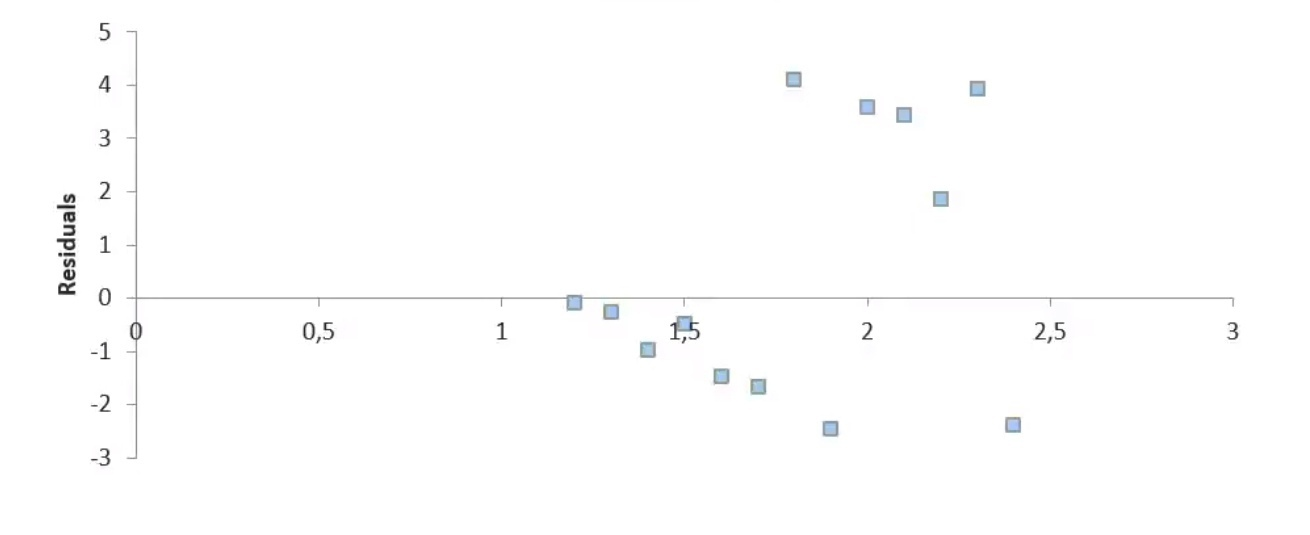
\includegraphics[width=0.35\textwidth]{graph2.png}
    \caption[Optional caption]{Residual plot}
    \label{fig:graph2}
\end{wrapfigure}

На графике можно выделить 2 группы. 

Если возьмем х примерно меньше 1,7, то остатки достаточно близко к нулю, в другой группе - существенно больше нуля. 

В левой группе дисперсия оказывается существенно меньше, чем в правой. 

\textit{Получили визуальную оценку гетероскедастичности данных.}

Чтобы избавиться от гетероскедастичности, можно попытаться воспользоваться альтернативными МНК, либо каким-то образом поработать с данными.

\section{Теорема Гаусса-Маркова}\label{sec:g-m}
\textbf{Теоремой Гаусса-Маркова} называется следующее утверждение: если условия применимости метода наименьших квадратов выполнены, то МНК-оценки являются несмещенными, эффективными, состоятельными, асимптотически нормальными. 

Что делать при невыполнении теоремы Гаусса-Маркова:
\begin{itemize}
    \item взять не сумму наименьших квадратов, а сумму наименьших абсолютных отклонений;
    \item рассмотреть взвешенные наименьшие квадраты;
\end{itemize}

\section{Маленькое число наблюдений}\label{sec:g-m}
\begin{itemize}
    \item В случае, когда число наблюдений велико, можно применить центральную предельную теорему: все доверительные интервалы и применение критериев обосновано. Важно, чтобы распределение ошибок было не важно каким, но не менялось; \\
    \item В случае малых объемов выборки (< 30) обязательно проверить, что остатки имеют нормальное распределение с одной и той же дисперсией;
\end{itemize}


\end{document}
